\documentclass[10pt]{article}
% Formato común del grupo (igual al informe de la Pregunta 3): carta, bloque 5.5 x 9 in, Times 10 pt,
% título 17 pt entre reglas, secciones "1." 12 pt negrita, subsecciones "3.1." 10 pt negrita, sin sangría.
\usepackage[letterpaper,textwidth=5.5in,textheight=9in,top=1in,footskip=30pt]{geometry}
\usepackage{mathptmx}
\usepackage[scaled=.92]{helvet}
\usepackage[utf8]{inputenc}
\usepackage[T1]{fontenc}
\usepackage{amsmath,amssymb}
\usepackage{graphicx}
\usepackage{booktabs}
\usepackage{xcolor}
\usepackage[hidelinks]{hyperref}
\usepackage{url}
\usepackage[numbers,sort&compress]{natbib}
\usepackage{microtype}
\usepackage{caption}
\usepackage{enumitem}
\usepackage{titlesec}
\usepackage{tikz}
\usetikzlibrary{arrows.meta}

\captionsetup{font=small,labelsep=colon,justification=centering}
\captionsetup[table]{skip=4pt}
\setlist{nosep,leftmargin=1.6em,topsep=2pt}
\setlength{\parindent}{0pt}
\setlength{\parskip}{5pt}
\renewcommand{\thesubsection}{\thesection.\arabic{subsection}}
\titleformat{\section}{\fontsize{12}{14}\bfseries}{\thesection.}{0.4em}{}
\titleformat{\subsection}{\normalsize\bfseries}{\thesubsection.}{0.4em}{}
\titlespacing*{\section}{0pt}{12pt}{4pt}
\titlespacing*{\subsection}{0pt}{8pt}{2pt}
\renewcommand{\figurename}{Figura}
\renewcommand{\tablename}{Tabla}
\renewcommand{\refname}{Referencias}
\setcitestyle{square}

\IfFileExists{generado/numeros.tex}{\newcommand{\BestRun}{E5b}
\newcommand{\BestLoss}{Dice}
\newcommand{\BestData}{dorado}
\newcommand{\Steps}{3000}
\newcommand{\IoUvalEone}{0.615}
\newcommand{\IoUvalEtwo}{0.598}
\newcommand{\IoUvalBest}{0.641}
\newcommand{\IoUtestBest}{0.663}
\newcommand{\FonetestBest}{0.798}
\newcommand{\PrectestBest}{0.821}
\newcommand{\RectestBest}{0.776}
\newcommand{\IoUbolBest}{0.572}
\newcommand{\IoUvalNoSkip}{0.634}
\newcommand{\IoUvalDepthThree}{0.641}
\newcommand{\MinutesTotal}{63}
\newcommand{\IoUotsuTest}{0.554}
\newcommand{\IoULima}{0.001}
\newcommand{\PrecLima}{0.001}
\newcommand{\RecLima}{0.006}
\newcommand{\FoneLima}{0.002}
\newcommand{\LxNPoligonos}{293}
\newcommand{\LxPctPoligonosDetectados}{1.7}
\newcommand{\LxKmInundadosEmsn}{6.0}
\newcommand{\LxKmEvaluables}{1708.8}
\newcommand{\LxPctAguaDentro}{0.1}
\newcommand{\LxPctAguaFuera}{1.1}
}{}
\newcommand{\fig}[2]{\IfFileExists{figuras/#1}{\includegraphics[#2]{figuras/#1}}{\fbox{\parbox{0.9\linewidth}{\centering\small Figura pendiente: \texttt{\detokenize{#1}}}}}}

\begin{document}
\thispagestyle{plain}
% ---------------------------------------------------------------- título
\begin{center}
\rule{\linewidth}{3pt}\par\vspace{10pt}
{\fontsize{17}{20.5}\selectfont\bfseries Pregunta 2\\
Mapeo de Inundaciones a partir de Radar Satelital\\ Sentinel-1 (U-Net)\par}
\vspace{8pt}\rule{\linewidth}{1pt}\par\vspace{18pt}
{\fontsize{12}{14}\selectfont\bfseries Abstract\par}
\end{center}
\vspace{-2pt}
{\leftskip=0.5in\rightskip=0.5in\parfillskip=0pt plus 1fil\noindent
Durante una inundación, las nubes inutilizan a los satélites ópticos justo cuando más se los necesita; el radar de Sentinel-1 las atraviesa. Implementamos desde cero una U-Net que segmenta el agua a partir de las bandas VV y VH, y la entrenamos con Sen1Floods11, que combina 446 chips etiquetados a mano con miles de etiquetas automáticas por umbral. En un estudio de ablación con presupuesto fijo, el mejor modelo (etiquetas doradas, pérdida Dice, profundidad 3) alcanza un IoU de agua de 0.663 en eventos vistos, frente a 0.554 del umbral de Otsu. Añadir etiquetas débiles no cambia ese resultado (0.640 frente a 0.641), pero en Bolivia, un evento no visto, eleva el IoU de 0.41 a 0.72. Construimos una región de prueba propia para el Perú con la escena Sentinel-1 del 17 de marzo de 2017 sobre Lima y la delineación de inundación EMSN038 de Copernicus. Allí el IoU cae a 0.001 en las siete variantes. Un diagnóstico físico muestra que la retrodispersión dentro de los polígonos ($-18.9$\,dB) está lejos de la del agua abierta ($-25.4$\,dB) y no aumenta al retirarse la inundación: la referencia óptica cartografía huellas de lodo vistas días después, no agua visible para el radar. Los errores propios del modelo se deben al suelo húmedo, la vegetación inundada, el doble rebote y la sombra de radar.\par}

% ===========================================================================
\section{Motivación}
\label{sec:intro}
Entre enero y marzo de 2017, el Niño costero provocó lluvias extraordinarias en la costa peruana. En Lima, una ciudad desértica donde casi nunca llueve, los ríos Rímac, Chillón y Huaycoloro se desbordaron y los huaicos afectaron Carapongo, Santa María de Huachipa, Cajamarquilla, Comas, Carabayllo y Puente Piedra. El Servicio de Gestión de Emergencias de Copernicus (EMS) respondió con la activación EMSN038, que delimitó en polígonos las zonas inundadas a partir de imágenes ópticas WorldView-2 del 18 y 21 de marzo \citep{emsn038}.

Ese tipo de cartografía es crítica en las horas siguientes al desastre, pero depende de imágenes ópticas que las nubes de tormenta suelen bloquear. El radar de apertura sintética (SAR) de Sentinel-1 \citep{torres2012} emite su propia señal de microondas, atraviesa las nubes y adquiere de noche. El agua tranquila se comporta como un espejo que refleja la señal lejos del satélite (retrodispersión baja, píxeles oscuros), mientras que el suelo rugoso, la vegetación y las construcciones devuelven más energía. Por eso el SAR es la herramienta de facto para el mapeo rápido de inundaciones.

Este trabajo implementa una U-Net \citep{ronneberger2015} para segmentar el agua en imágenes Sentinel-1 y atiende las tres dificultades del enunciado: cómo combinar pocas etiquetas expertas con muchas etiquetas automáticas ruidosas, qué decisiones de pérdida y arquitectura funcionan con un fuerte desbalance de clases, y qué tan bien generaliza el modelo a una región nunca vista, para lo cual construimos una región de prueba propia en Lima.

% ===========================================================================
\section{Trabajos Relacionados}
\label{sec:rel}
\citet{long2015} mostraron que una red de clasificación puede convertirse en un predictor denso reemplazando sus capas totalmente conectadas por convoluciones. La U-Net \citep{ronneberger2015} añadió un camino de expansión simétrico y conexiones de salto por concatenación, que devuelven al decodificador la información espacial fina que el codificador pierde al reducir resolución, y propuso entrenar con muy pocas imágenes gracias a deformaciones elásticas y a una pérdida ponderada que enfatiza los bordes. Entre sus variantes, V-Net \citep{milletari2016} introdujo la pérdida Dice para el desbalance de clases, U-Net++ \citep{zhou2018} anidó los saltos, Attention U-Net \citep{oktay2018} les añadió compuertas de atención y nnU-Net \citep{isensee2021} autoconfigura la arquitectura para cada dataset.

En el mapeo de inundaciones con SAR, el enfoque clásico umbraliza la retrodispersión, típicamente con el método de Otsu \citep{otsu1979}, y lo integra en cadenas automáticas como la de \citet{twele2016}. Estos métodos no requieren entrenamiento, pero confunden el agua con otras superficies oscuras y fallan donde el agua no es lisa. \citet{bonafilia2020} publicaron Sen1Floods11, el primer dataset global para entrenar redes en este problema, y observaron que las redes entrenadas con abundantes etiquetas automáticas podían superar a las entrenadas solo con las escasas etiquetas manuales. Como referencia de agua permanente usamos el mapa global de \citet{pekel2016}, y obtenemos las escenas con Google Earth Engine \citep{gorelick2017}.

% ===========================================================================
\section{Metodología}
\label{sec:metodo}
\subsection{Datos y particiones}
\label{sec:datos}
Sen1Floods11 contiene 11 eventos de inundación en seis continentes, en chips de $512\times512$ píxeles a 10\,m (EPSG:4326) con las bandas VV y VH en dB \citep{bonafilia2020}. Usamos los 446 chips con etiqueta dorada (agua, no agua o sin datos, anotada por expertos) con la partición oficial, y como fuente débil una muestra aleatoria reproducible de 1\,500 de los 4\,160 chips etiquetados por umbral de Otsu sobre VH, sin Bolivia (Tabla~\ref{tab:datos}). El agua es el 9.5\,\% de los píxeles válidos del entrenamiento dorado, pero el 17.8\,\% en las etiquetas débiles: el umbral tiende a sobreestimarla. Igual que los autores, recortamos los dB a $[-50,1]$, los escalamos a $[0,1]$ y estandarizamos cada banda con estadísticas calculadas solo sobre el entrenamiento dorado. Los píxeles sin datos se excluyen de la pérdida y de las métricas.

\begin{table}[h]
\centering\small
\caption{Conjuntos usados. Todas las particiones de Sen1Floods11 son las oficiales.}
\label{tab:datos}
\begin{tabular}{llrl}
\toprule
\textbf{Conjunto} & \textbf{Etiqueta} & \textbf{Chips} & \textbf{Uso} \\
\midrule
train & dorada & 252 & Entrenar \\
valid & dorada & 89 & Elegir el mejor punto y la configuración \\
test & dorada & 90 & Entregable 3 (eventos vistos) \\
Bolivia & dorada & 15 & Evento no visto (referencia interna) \\
débil & Otsu sobre VH & 1\,500 & Ablación (a) \\
Lima, 17-mar-2017 & EMSN038 & escena + chips & Entregable 4 (Perú) \\
\bottomrule
\end{tabular}
\end{table}

Para la región del Perú buscamos en ASF Vertex las escenas Sentinel-1 GRD IW de doble polarización sobre Lima entre el 10 y el 31 de marzo de 2017 y encontramos tres: 10 de marzo (otra pasada, antes del evento), 17 de marzo a las 10:38 UTC (Sentinel-1B, órbita relativa 171, descendente) y 29 de marzo (misma órbita). La del 17 coincide con el día de los desbordes en Huachipa y Carapongo y precede en un día a la imagen óptica de EMSN038, por lo que es la escena de prueba. La obtuvimos de Earth Engine (\texttt{COPERNICUS/S1\_GRD}), con la misma calibración, corrección de terreno y conversión a dB que Sen1Floods11, y la remuestreamos a su grilla ($8.98\times10^{-5}$\,°), tanto como escena completa como en chips de $512\times512$. Como etiqueta usamos la capa de extensión de inundación de EMSN038 (\texttt{DamAssess\_A}, obtenida por análisis de objetos sobre la imagen óptica) restringida a lo observado a lo largo de los ríos (\texttt{source = river}, 660 polígonos, 6.34\,km²), y excluimos la extensión extrapolada hasta la cota máxima del agua. Solo se evalúan los píxeles dentro del área de interés de EMSN038, en tierra firme y que no son agua permanente según JRC \citep{pekel2016} (ocurrencia $\geq50\,\%$). Estas etiquetas no se generaron con el mismo criterio que las doradas: provienen de imágenes ópticas de mayor resolución y de fechas posteriores a la escena SAR, por lo que las tratamos como una supervisión débil propia y no como verdad de terreno.

\subsection{Modelo y entrenamiento (Entregable 1)}
\label{sec:modelo}
\begin{figure}[t]
\centering
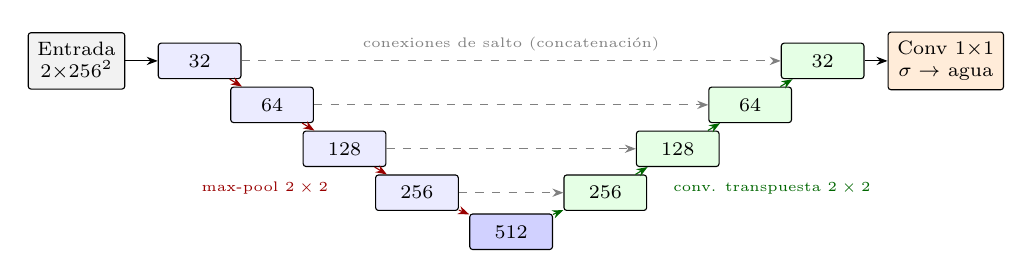
\begin{tikzpicture}[x=0.92cm,y=0.62cm,
  blk/.style={draw,rounded corners=1pt,minimum width=1.05cm,minimum height=0.45cm,font=\scriptsize,align=center,fill=#1},
  blk/.default=white, >={Stealth[length=4pt]}]
\node[blk=gray!10] (in) at (0,0) {Entrada\\2$\times$256$^2$};
\node[blk=blue!8] (e0) at (1.7,0) {32};
\node[blk=blue!8] (e1) at (2.7,-0.9) {64};
\node[blk=blue!8] (e2) at (3.7,-1.8) {128};
\node[blk=blue!8] (e3) at (4.7,-2.7) {256};
\node[blk=blue!18] (b) at (6.0,-3.5) {512};
\node[blk=green!10] (d3) at (7.3,-2.7) {256};
\node[blk=green!10] (d2) at (8.3,-1.8) {128};
\node[blk=green!10] (d1) at (9.3,-0.9) {64};
\node[blk=green!10] (d0) at (10.3,0) {32};
\node[blk=orange!15] (out) at (12.0,0) {Conv 1$\times$1\\$\sigma\to$ agua};
\draw[->] (in)--(e0); \draw[->] (d0)--(out);
\foreach \a/\c in {e0/e1,e1/e2,e2/e3,e3/b} \draw[->,red!60!black] (\a)--(\c);
\foreach \a/\c in {b/d3,d3/d2,d2/d1,d1/d0} \draw[->,green!40!black] (\a)--(\c);
\foreach \a/\c in {e0/d0,e1/d1,e2/d2,e3/d3} \draw[->,dashed,gray] (\a)--(\c);
\node[font=\tiny,gray] at (6.0,0.35) {conexiones de salto (concatenación)};
\node[font=\tiny,red!60!black] at (2.6,-2.6) {max-pool $2\times2$};
\node[font=\tiny,green!40!black] at (9.6,-2.6) {conv. transpuesta $2\times2$};
\end{tikzpicture}
\caption{U-Net implementada (base 32, profundidad 4, 7.76\,M parámetros; la variante de profundidad 3 elimina el nivel de 256 canales). Cada bloque aplica dos convoluciones $3\times3$ con \emph{padding}, BatchNorm y ReLU.}
\label{fig:arq}
\end{figure}

Implementamos la U-Net desde cero en PyTorch, sin bibliotecas de segmentación, siguiendo a \citet{ronneberger2015} con tres cambios hoy estándar: \emph{padding} de 1 (salida del mismo tamaño que la entrada), BatchNorm \citep{ioffe2015} e inicialización de He \citep{he2015} (Figura~\ref{fig:arq}). La entrada tiene dos canales (VV, VH) y la salida, un logit de agua por píxel; para dos clases, sigmoide con entropía cruzada binaria equivale a softmax con dos logits. Las decisiones documentadas son:
\begin{itemize}
\item \textbf{Funciones de pérdida:} BCE; Dice suave \citep{milletari2016}, $\mathcal{L}_{D}=1-\tfrac{2\sum p\,y+1}{\sum p+\sum y+1}$; su suma BCE + Dice; y BCE con peso en bordes, adaptación del mapa de pesos de U-Net, $w(x)=1+5\,(G_{\sigma=3} * B)(x)$, donde $B$ es el borde agua/no agua.
\item \textbf{Aumento de datos:} recortes aleatorios de $256\times256$, rotaciones de 90°, volteos y deformaciones elásticas como en U-Net (grilla $3\times3$, $\sigma=10$\,px). Sin ajustes de brillo ni contraste, porque en SAR la intensidad es la señal física.
\item \textbf{Mezcla de etiquetas:} al añadir las débiles se muestrea 50\,\% de chips dorados y 50\,\% de débiles, para que las 1\,500 etiquetas ruidosas no dominen a las 252 expertas.
\item \textbf{Optimización:} AdamW \citep{loshchilov2019} con política OneCycle \citep{smith2019} (tasa máxima $2\times10^{-3}$), lote de 16, precisión mixta y 3\,000 pasos en todas las corridas. Con el mismo presupuesto, añadir datos no gana solo por entrenar más. Cada 250 pasos se evalúa en validación y se guarda el mejor punto según el IoU de agua.
\end{itemize}
Entrenamos en Google Colab con una GPU T4; cada corrida tarda unos 9 minutos.

\subsection{Evaluación}
Para la clase agua reportamos IoU, F1, precisión, recall, omisión y comisión \citep{bonafilia2020}, y el IoU de dos formas: agregado sobre todos los píxeles y promedio por chip, que es la métrica de los autores del dataset. Todas las decisiones de la ablación se toman con validación; prueba, Bolivia y Lima se reportan sin usarlas para elegir. La escena de Lima ($\sim$5\,500$\times$4\,000 píxeles) se predice con la estrategia \emph{overlap-tile} de U-Net: mosaicos de 512 píxeles con 64 de margen, de los que solo se conserva el centro, con relleno por reflexión en los bordes. Para separar el error del modelo del de la referencia, comparamos además la retrodispersión dentro y fuera de los polígonos de EMSN038, el cambio entre el 17 y el 29 de marzo y un umbral de Otsu calculado sobre la propia escena.

% ===========================================================================
\section{Resultados}
\label{sec:res}
\subsection{Estudio de ablación (Entregable 2)}
\begin{table}[t]
\centering\small
\caption{Estudio de ablación. Todas las corridas usan el mismo presupuesto (3000 pasos, lote 16, recortes de 256\,px). La selección se hace con el IoU de agua en \emph{validación} (el mejor, en negrita); las columnas de prueba y Bolivia se reportan solo como referencia.}
\label{tab:ablacion}
\setlength{\tabcolsep}{4pt}
\resizebox{\linewidth}{!}{\begin{tabular}{lllcrcccc}
\toprule
\textbf{Corrida} & \textbf{Datos} & \textbf{Pérdida} & \textbf{Arquitectura} & \textbf{Parám. (M)} & \textbf{IoU val} & \textbf{IoU test} & \textbf{F1 test} & \textbf{IoU Bolivia} \\
\midrule
E1 & dorado & BCE & con saltos, prof. 4 & 7.76 & 0.615 & 0.640 & 0.781 & 0.408 \\
E2 & dorado + débil & BCE & con saltos, prof. 4 & 7.76 & 0.598 & 0.641 & 0.781 & 0.716 \\
E3 & dorado & Dice & con saltos, prof. 4 & 7.76 & 0.630 & 0.661 & 0.796 & 0.615 \\
E4 & dorado & BCE + Dice & con saltos, prof. 4 & 7.76 & 0.621 & 0.656 & 0.792 & 0.518 \\
E6 & dorado & BCE con peso en bordes & con saltos, prof. 4 & 7.76 & 0.624 & 0.665 & 0.799 & 0.598 \\
E5a & dorado & Dice & sin saltos, prof. 4 & 6.98 & 0.634 & 0.649 & 0.787 & 0.594 \\
E5b & dorado & Dice & con saltos, prof. 3 & 1.93 & \textbf{0.641} & 0.663 & 0.798 & 0.572 \\
\bottomrule
\end{tabular}}
\end{table}

La Tabla~\ref{tab:ablacion} resume las siete corridas, que tomaron en total 63 minutos, y la Figura~\ref{fig:curvas}, sus curvas de aprendizaje.

\textbf{(a) Etiquetas doradas frente a doradas + débiles.} En validación, entrenar solo con los 252 chips dorados (E1, IoU 0.615) supera ligeramente a añadir las etiquetas débiles (E2, 0.598), y en prueba ambas quedan empatadas (0.640 frente a 0.641). La diferencia aparece fuera de distribución: en Bolivia, E2 alcanza un IoU de 0.716, frente a 0.408 de E1. Casi todo el cambio está en el recall (0.788 frente a 0.430), porque la precisión es la misma ($\approx$0.89). El modelo entrenado solo con etiquetas expertas aprende un criterio de agua conservador, ajustado a los diez eventos vistos, y en una región nueva deja de detectar gran parte del agua. Las etiquetas de Otsu, más abundantes, más diversas y sesgadas hacia marcar más agua, corrigen ese sesgo. Así se concilian las dos tesis: en distribución bastan pocas etiquetas buenas con aumento agresivo, como propone U-Net, mientras que para generalizar importa la cantidad y diversidad de la supervisión, como observaron \citet{bonafilia2020}.

\textbf{(b) Función de pérdida.} Las tres alternativas a la BCE pura tienen un IoU de validación muy parecido: Dice (E3) 0.630, BCE con peso en bordes (E6) 0.624 y BCE + Dice (E4) 0.621. En prueba el orden cambia (E6 0.665, E3 0.661, E4 0.656). Como el IoU de validación oscila hasta $\pm$0.05 entre evaluaciones (Figura~\ref{fig:curvas}), más que la distancia entre ellas, no hay un ganador claro. La señal consistente es que las tres superan a la BCE pura en validación, en prueba ($+0.016$ a $+0.025$) y sobre todo en Bolivia (0.52 a 0.62 frente a 0.41). Con solo 9.5\,\% de píxeles de agua, la BCE produce un modelo conservador (precisión 0.886, recall 0.669 en validación); Dice y el peso en bordes ceden algo de precisión a cambio de recall (0.70 a 0.72). Por su IoU de validación, Dice pasa a la etapa (c).

\textbf{(c) Arquitectura.} Ninguna de las dos variantes empeora la validación. La profundidad 3 (E5b), con un modelo cuatro veces más pequeño (1.93\,M frente a 7.76\,M parámetros), obtiene el mejor IoU de validación del estudio (0.641) e iguala en prueba a la red completa (0.663 frente a 0.661): con 252 chips de entrenamiento, el límite son los datos y no la capacidad, y a 10\,m por píxel tres reducciones bastan para reconocer cuerpos de agua. Quitar las conexiones de salto (E5a) tampoco degrada el IoU de validación, a diferencia del experimento de la Clase 9, pero cambia el tipo de error: la precisión cae de 0.832 a 0.792 en validación y el IoU de prueba baja de 0.661 a 0.649, porque sin la información fina de los saltos el contorno del agua se predice engrosado. El efecto es pequeño porque el IoU agregado lo dominan cuerpos de agua grandes y homogéneos. El modelo final, elegido por validación, es E5b (dorado, Dice, profundidad 3).

\begin{figure}[t]
\centering\fig{fig_curvas.png}{width=\linewidth}
\caption{Pérdida de entrenamiento (izq.) e IoU de agua en validación (der.) de las siete corridas. La oscilación a mitad del entrenamiento coincide con el máximo de la tasa de aprendizaje de OneCycle.}
\label{fig:curvas}
\end{figure}

\subsection{Evaluación en distribución (Entregable 3)}
\begin{table}[t]
\centering\small
\caption{Clase \emph{agua}: modelo final (E5b) frente a la línea base clásica (umbral de Otsu sobre VH). \emph{test}: chips dorados de los eventos vistos en entrenamiento; \emph{bolivia}: evento nunca visto. IoU agregado sobre todos los píxeles válidos e IoU promedio por chip (métrica de los autores del dataset).}
\label{tab:eval}
\setlength{\tabcolsep}{4pt}
\resizebox{\linewidth}{!}{\begin{tabular}{lccccccc}
\toprule
\textbf{Conjunto} & \textbf{IoU} & \textbf{IoU/chip} & \textbf{F1} & \textbf{Precisión} & \textbf{Recall} & \textbf{Omisión} & \textbf{Comisión} \\
\midrule
U-Net (test) & 0.663 & 0.388 & 0.798 & 0.821 & 0.776 & 0.224 & 0.179 \\
Otsu VH (test) & 0.554 & 0.332 & 0.713 & 0.682 & 0.748 & 0.252 & 0.318 \\
U-Net (bolivia) & 0.572 & 0.352 & 0.728 & 0.884 & 0.618 & 0.382 & 0.116 \\
Otsu VH (bolivia) & 0.718 & 0.474 & 0.836 & 0.803 & 0.870 & 0.130 & 0.197 \\
\bottomrule
\end{tabular}}
\end{table}

En los 90 chips de prueba, el modelo final obtiene un IoU de 0.663, F1 de 0.798, precisión de 0.821 y recall de 0.776 (Tabla~\ref{tab:eval}). Frente al umbral de Otsu, sube el IoU de 0.554 a 0.663 y reduce la comisión de 0.318 a 0.179 sin perder recall: aprende a no confundir con agua otras superficies oscuras que el umbral marca sin distinción. La matriz de confusión (Figura~\ref{fig:cm}) clasifica bien el 97.6\,\% de los píxeles de no agua y el 77.6\,\% de los de agua, de modo que el error dominante es la omisión: uno de cada cuatro píxeles de agua queda sin detectar. El IoU promedio por chip (0.388) es mucho menor que el agregado porque muchos chips contienen muy poca agua, y en ellos unos pocos píxeles mal clasificados llevan el IoU del chip cerca de cero. En Bolivia la relación se invierte: Otsu (0.718) supera a la U-Net (0.572), cuyo recall cae a 0.618, porque el umbral se recalcula con el histograma de cada escena y se adapta a la nueva región, mientras que la red aplica la relación aprendida en otros eventos.

\begin{figure}[t]
\centering\fig{fig_matriz_confusion.png}{width=0.8\linewidth}
\caption{Matriz de confusión del modelo final en la prueba en distribución: conteos en millones de píxeles (izq.) y normalizada por fila, es decir, recall por clase (der.).}
\label{fig:cm}
\end{figure}

\subsection{Generalización geográfica al Perú (Entregable 4)}
\label{sec:lima}
\begin{table}[t]
\centering\small
\caption{Generalización geográfica: el modelo entrenado solo con Sen1Floods11 evaluado sobre Lima (Sentinel-1 del 17-mar-2017 contra la delineación EMSN038), frente a la prueba en distribución.}
\label{tab:lima}
\setlength{\tabcolsep}{4pt}
\resizebox{\linewidth}{!}{\begin{tabular}{lccccccc}
\toprule
\textbf{Conjunto} & \textbf{IoU} & \textbf{IoU/chip} & \textbf{F1} & \textbf{Precisión} & \textbf{Recall} & \textbf{Omisión} & \textbf{Comisión} \\
\midrule
Prueba en distribución & 0.663 & 0.388 & 0.798 & 0.821 & 0.776 & 0.224 & 0.179 \\
Lima 17-mar-2017 (EMSN038) & 0.001 & 0.010 & 0.002 & 0.001 & 0.006 & 0.994 & 0.999 \\
Brecha (Lima $-$ dist.) & -0.662 & -0.379 & -0.796 & -0.820 & -0.770 & 0.770 & 0.820 \\
\bottomrule
\end{tabular}}
\end{table}

Sobre Lima, el modelo final obtiene un IoU de 0.001 (precisión 0.001, recall 0.006), frente a 0.663 en distribución (Tabla~\ref{tab:lima}), y solo detecta agua en el 1.7\,\% de los 293 polígonos de EMSN038 evaluables (con el criterio de al menos 25\,\% de su área). El área evaluable es de 1\,709\,km², de los cuales 5.98\,km² están marcados como inundados. Las siete corridas fallan por igual, con IoU entre 0.0003 y 0.013 (Tabla~\ref{tab:limatodas}), sin relación con su desempeño en validación o en Bolivia: E2, la mejor en Bolivia, es la peor en Lima. Que ninguna decisión de la ablación cambie el resultado sugiere una causa común ajena al modelo.

\begin{table}[t]
\centering\small
\caption{Izquierda: IoU de cada corrida en validación, prueba, Bolivia y Lima. Derecha: mediana de VH (dB) dentro de la zona de agua o inundada y en el resto, cambio entre fechas y umbral de Otsu sobre la escena de Lima.}
\label{tab:limatodas}
\begin{minipage}[t]{0.50\linewidth}\centering\vspace{0pt}
\begin{tabular}{lcccc}
\toprule
\textbf{Corrida} & \textbf{Val} & \textbf{Test} & \textbf{Bolivia} & \textbf{Lima} \\
\midrule
E1 & 0.615 & 0.640 & 0.408 & 0.007 \\
E2 & 0.598 & 0.641 & 0.716 & 0.000 \\
E3 & 0.630 & 0.661 & 0.615 & 0.008 \\
E4 & 0.621 & 0.656 & 0.518 & 0.007 \\
E6 & 0.624 & 0.665 & 0.598 & 0.013 \\
E5a & 0.634 & 0.649 & 0.594 & 0.003 \\
E5b & 0.641 & 0.663 & 0.572 & 0.001 \\
\bottomrule
\end{tabular}
\end{minipage}\hfill
\begin{minipage}[t]{0.47\linewidth}\centering\vspace{0pt}
\begin{tabular}{lcc}
\toprule
\textbf{VH (dB)} & \textbf{Agua / inund.} & \textbf{Resto} \\
\midrule
Sen1Floods11 & $-25.4$ & $-16.0$ \\
Lima 17-mar & $-18.9$ & $-17.5$ \\
Lima 29-mar & $-19.3$ & $-17.4$ \\
\midrule
\multicolumn{3}{l}{Cambio 29$-$17 mar: $-0.41$ dentro, $+0.05$ fuera} \\
\multicolumn{3}{l}{Otsu en Lima: IoU 0.005, P 0.005, R 0.725} \\
\bottomrule
\end{tabular}
\end{minipage}
\end{table}

Para comprobar si el radar veía agua donde EMSN038 marca inundación, comparamos la retrodispersión dentro y fuera de los polígonos (Tabla~\ref{tab:limatodas}, Figura~\ref{fig:hist}). Dentro, la mediana de VH es $-18.9$\,dB, apenas 1.4\,dB más oscura que el resto de Lima y lejos de los $-25.4$\,dB del agua de Sen1Floods11. Solo el 35\,\% de esos píxeles está por debajo de $-20$\,dB, frente al 78\,\% del agua de entrenamiento. Si el 17 de marzo hubiera habido una lámina de agua que luego se retiró, la señal debería haber subido varios dB hacia el 29; dentro de los polígonos, en cambio, bajó 0.41\,dB, y afuera no cambió. Por último, un umbral de Otsu sobre la propia escena, sin entrenamiento, recupera el 72\,\% de los píxeles marcados pero con precisión 0.005: la leve oscuridad de los polígonos no se distingue del resto de la ciudad ni del desierto. La escena SAR del 17 de marzo no muestra agua abierta donde EMSN038 marca inundación.

\begin{figure}[t]
\centering
\fig{fig_lima_huachipa.png}{width=\linewidth}\\[2pt]
\fig{fig_lima_comas.png}{width=\linewidth}
\caption{Lima, 17 y 29 de marzo de 2017: Huachipa--Carapongo (arriba) y Comas--Carabayllo (abajo). De izquierda a derecha: VH (dB), predicción del 17 de marzo, error frente a EMSN038 (oscuro = acierto, rojo = falso positivo, azul = falso negativo) y predicción del 29 de marzo. En amarillo, los polígonos de EMSN038.}
\label{fig:lima}
\end{figure}

\begin{figure}[t]
\centering\fig{fig_lima_histogramas.png}{width=\linewidth}
\caption{Diagnóstico físico de Lima. Izquierda: distribución de VH dentro de los polígonos de EMSN038 (rojo), en el resto del área evaluable (negro) y en el agua y no agua de Sen1Floods11 (azul y gris); la línea discontinua es el umbral de Otsu de la escena ($-17.2$\,dB). Derecha: cambio de VH entre el 17 y el 29 de marzo.}
\label{fig:hist}
\end{figure}

\subsection{Errores característicos del SAR (Entregable 5)}
\label{sec:errores}
Los chips de prueba con más errores (Figura~\ref{fig:errores}) y la escena de Lima muestran cinco tipos de error:
\begin{itemize}
\item \textbf{Superficies lisas no inundadas (falsos positivos):} en \texttt{Pakistan\_70625} la etiqueta solo marca un canal, pero el modelo predice agua en parcelas oscuras: campos regados, suelo húmedo o desnudo, cuya superficie lisa también refleja la señal lejos del sensor. Es la confusión entre suelo húmedo y agua abierta, que el SAR por sí solo no resuelve.
\item \textbf{Vegetación inundada (falsos negativos):} en \texttt{Pakistan\_849790} e \texttt{India\_747992}, grandes zonas etiquetadas como agua aparecen en gris medio y no en negro, porque hay agua bajo cultivos o vegetación. La señal rebota entre el agua y los tallos y vuelve con más energía, así que el agua no se ve oscura. Es la principal fuente de omisión.
\item \textbf{Doble rebote urbano y bordes:} en \texttt{Spain\_7387658} se mezclan falsos positivos finos en los bordes de parcelas y caminos con falsos negativos dentro del casco urbano, donde el agua alrededor de las edificaciones produce un doble rebote brillante.
\item \textbf{Sombra de radar:} en Lima, la mayoría de los falsos positivos son manchas en las laderas de los cerros de Huachipa, Cajamarquilla y Carabayllo (Figura~\ref{fig:lima}). Son las pendientes opuestas al sensor en órbita descendente, que no reciben señal y se ven tan oscuras como el agua. Los eventos de Sen1Floods11 están en llanuras, por lo que el modelo no aprendió a descartarlas.
\item \textbf{Errores de la propia etiqueta:} en \texttt{Ghana\_866994} la etiqueta dorada son polígonos suavizados con grandes zonas sin datos por nubes en la imagen óptica de referencia, y en \texttt{USA\_595451} e \texttt{India\_399883} hay zonas muy oscuras junto al río que no se marcaron como agua. Parte de los errores son desacuerdos con una referencia imperfecta.
\end{itemize}

\begin{figure}[t]
\centering
\fig{fig_errores_FP.png}{width=0.49\linewidth}\hfill
\fig{fig_errores_FN.png}{width=0.49\linewidth}
\caption{Chips de prueba con más falsos positivos (izq.) y más falsos negativos (der.). Columnas: VV, VH, etiqueta dorada y mapa de error (gris oscuro = acierto, rojo = falso positivo, azul = falso negativo).}
\label{fig:errores}
\end{figure}

% ===========================================================================
\section{Discusión}
\label{sec:disc}
\subsection{¿Qué mide la brecha de Lima?}
Contrastamos con la evidencia las hipótesis sobre la caída de 0.663 a 0.001:
\begin{itemize}
\item \textbf{Desajuste temporal y de sensor de la referencia (respaldada):} EMSN038 delinea por análisis de objetos sobre imágenes ópticas del 18 y 21 de marzo, mientras que el SAR es del 17 de marzo a las 05:38 hora local. Los huaicos y desbordes duran horas, y lo que la imagen óptica registra días después son huellas de la inundación. Que la retrodispersión no suba entre el 17 y el 29 de marzo dentro de los polígonos indica que el 17 tampoco había una lámina de agua que luego se retirara.
\item \textbf{Lodo frente a agua abierta (respaldada):} el VH dentro de los polígonos tiene una distribución estrecha centrada en $-18.9$\,dB, típica de cauces de grava, barro y depósitos de huaico, no de agua abierta ($-25$\,dB). Los huaicos son flujos de lodo de superficie rugosa, muy distintos de las llanuras aluviales de Sen1Floods11.
\item \textbf{Escala y desbalance extremo (respaldada):} la inundación delineada son franjas de 100 a 200\,m a lo largo de los cauces, el 0.35\,\% del área evaluable frente al 9.5\,\% de Sen1Floods11. Con 285 píxeles secos por cada inundado, una tasa de falsos positivos de 1.65\,\% basta para que estos superen a los aciertos, aunque el modelo acierte el 98\,\% del área seca.
\item \textbf{Geometría del radar (respaldada):} las sombras de radar en el relieve abrupto del valle del Rímac explican la mayoría de los falsos positivos, y no hay relieve parecido en el entrenamiento.
\item \textbf{Cobertura urbana y doble rebote (no verificable):} las zonas afectadas incluyen áreas urbanas donde el agua entre edificaciones devolvería una señal brillante, pero con esta referencia no es posible aislar el efecto.
\end{itemize}
La brecha mide sobre todo el desacuerdo entre dos definiciones de inundación: la del modelo y de Sen1Floods11, que es agua abierta visible para el radar en el instante de adquisición, y la de EMSN038, que es el área afectada cartografiada en imágenes ópticas días después. No puede atribuirse solo al modelo, porque un método sin entrenamiento también fracasa y la señal no contiene agua donde la referencia la marca.

\subsection{Limitaciones}
\begin{itemize}
\item Cada configuración se entrenó con una sola semilla. Diferencias de una o dos centésimas de IoU están dentro de la variabilidad esperable y no son concluyentes; lo correcto sería repetir cada corrida con 3 a 5 semillas.
\item Usamos 1\,500 de los 4\,160 chips débiles y el mismo número de pasos en todas las corridas. Con más cómputo, las etiquetas débiles podrían rendir más, por ejemplo como preentrenamiento seguido de ajuste fino con las doradas, alternativa que no exploramos.
\item La referencia de Lima no es verdad de terreno para la fecha del SAR; separar el error del modelo del de la referencia exigiría etiquetar a mano la propia escena SAR.
\item No realizamos la fusión opcional con Sentinel-2, y usamos un umbral fijo de 0.5 sobre la probabilidad; calibrarlo por región podría reducir parte de la brecha.
\end{itemize}

% ===========================================================================
\section{Conclusiones}
\begin{itemize}
\item La U-Net propia, con etiquetas doradas, pérdida Dice y profundidad 3, alcanza un IoU de agua de 0.663 en eventos vistos y supera al umbral de Otsu (0.554), sobre todo porque reduce la comisión.
\item Las pérdidas que atienden el desbalance superan a la BCE pura, y una red cuatro veces más pequeña rinde igual que la completa: con 252 chips, el límite son los datos.
\item Las etiquetas débiles no mejoran el rendimiento en distribución, pero en un evento no visto elevan el IoU de 0.41 a 0.72 al corregir el recall. Elegir el modelo solo con la validación en distribución descarta la opción que mejor generaliza.
\item En Lima ninguna variante funciona (IoU $\leq$0.013). La brecha se explica sobre todo por la referencia: la escena SAR del 17 de marzo no contiene agua abierta en los polígonos de EMSN038, que cartografían huellas de lodo vistas días después. Lo atribuible al modelo son los falsos positivos por sombra de radar en el relieve abrupto.
\end{itemize}
Como trabajo futuro proponemos etiquetar a mano un evento peruano sobre la propia escena SAR, añadir el modelo de elevación (pendiente y máscara de sombra) como entrada o filtro y, para huaicos, detectar el cambio entre una escena previa y una posterior de la misma órbita en lugar de buscar agua en una sola fecha.

% ===========================================================================
\section{Material complementario}
El código, el notebook, las tablas de resultados y las figuras están en el repositorio\\ \url{https://github.com/SebastianVillanueva/p2-parcial-sebastian}.\\ Todo el flujo se ejecuta con \texttt{python run\_all.py -{}-ee-project <ID>}, como se describe en el README, y las etiquetas de EMSN038 se descargan automáticamente.

% ===========================================================================
{\small
\renewcommand{\section}[2]{\vspace{6pt}{\fontsize{12}{14}\bfseries Referencias\par}\vspace{2pt}}
\begin{thebibliography}{99}
\setlength{\itemsep}{1pt}
\bibitem[Copernicus EMS(2017)]{emsn038} Copernicus Emergency Management Service (2017). EMSN038: Post-disaster situation analyses of flood and landslides in Lima, Peru. \url{https://mapping.emergency.copernicus.eu/activations/EMSN038/}
\bibitem[Torres et~al.(2012)]{torres2012} Torres, R., Snoeij, P., Geudtner, D., et al. (2012). GMES Sentinel-1 mission. \emph{Remote Sensing of Environment}, 120, 9--24.
\bibitem[Ronneberger et~al.(2015)]{ronneberger2015} Ronneberger, O., Fischer, P., \& Brox, T. (2015). U-Net: Convolutional networks for biomedical image segmentation. \emph{Medical Image Computing and Computer-Assisted Intervention (MICCAI)}, 234--241.
\bibitem[Long et~al.(2015)]{long2015} Long, J., Shelhamer, E., \& Darrell, T. (2015). Fully convolutional networks for semantic segmentation. \emph{IEEE Conference on Computer Vision and Pattern Recognition (CVPR)}, 3431--3440.
\bibitem[Milletari et~al.(2016)]{milletari2016} Milletari, F., Navab, N., \& Ahmadi, S.-A. (2016). V-Net: Fully convolutional neural networks for volumetric medical image segmentation. \emph{International Conference on 3D Vision (3DV)}, 565--571.
\bibitem[Zhou et~al.(2018)]{zhou2018} Zhou, Z., Siddiquee, M. M. R., Tajbakhsh, N., \& Liang, J. (2018). UNet++: A nested U-Net architecture for medical image segmentation. \emph{Deep Learning in Medical Image Analysis (DLMIA)}, 3--11.
\bibitem[Oktay et~al.(2018)]{oktay2018} Oktay, O., Schlemper, J., Le Folgoc, L., et al. (2018). Attention U-Net: Learning where to look for the pancreas. \emph{Medical Imaging with Deep Learning (MIDL)}.
\bibitem[Isensee et~al.(2021)]{isensee2021} Isensee, F., Jaeger, P. F., Kohl, S. A. A., Petersen, J., \& Maier-Hein, K. H. (2021). nnU-Net: A self-configuring method for deep learning-based biomedical image segmentation. \emph{Nature Methods}, 18, 203--211.
\bibitem[Otsu(1979)]{otsu1979} Otsu, N. (1979). A threshold selection method from gray-level histograms. \emph{IEEE Transactions on Systems, Man, and Cybernetics}, 9(1), 62--66.
\bibitem[Twele et~al.(2016)]{twele2016} Twele, A., Cao, W., Plank, S., \& Martinis, S. (2016). Sentinel-1-based flood mapping: A fully automated processing chain. \emph{International Journal of Remote Sensing}, 37(13), 2990--3004.
\bibitem[Bonafilia et~al.(2020)]{bonafilia2020} Bonafilia, D., Tellman, B., Anderson, T., \& Issenberg, E. (2020). Sen1Floods11: A georeferenced dataset to train and test deep learning flood algorithms for Sentinel-1. \emph{IEEE/CVF Conference on Computer Vision and Pattern Recognition Workshops (CVPRW)}, 210--211.
\bibitem[Pekel et~al.(2016)]{pekel2016} Pekel, J.-F., Cottam, A., Gorelick, N., \& Belward, A. S. (2016). High-resolution mapping of global surface water and its long-term changes. \emph{Nature}, 540, 418--422.
\bibitem[Gorelick et~al.(2017)]{gorelick2017} Gorelick, N., Hancher, M., Dixon, M., Ilyushchenko, S., Thau, D., \& Moore, R. (2017). Google Earth Engine: Planetary-scale geospatial analysis for everyone. \emph{Remote Sensing of Environment}, 202, 18--27.
\bibitem[Ioffe y Szegedy(2015)]{ioffe2015} Ioffe, S., \& Szegedy, C. (2015). Batch normalization: Accelerating deep network training by reducing internal covariate shift. \emph{International Conference on Machine Learning (ICML)}, 448--456.
\bibitem[He et~al.(2015)]{he2015} He, K., Zhang, X., Ren, S., \& Sun, J. (2015). Delving deep into rectifiers: Surpassing human-level performance on ImageNet classification. \emph{IEEE International Conference on Computer Vision (ICCV)}, 1026--1034.
\bibitem[Loshchilov y Hutter(2019)]{loshchilov2019} Loshchilov, I., \& Hutter, F. (2019). Decoupled weight decay regularization. \emph{International Conference on Learning Representations (ICLR)}.
\bibitem[Smith y Topin(2019)]{smith2019} Smith, L. N., \& Topin, N. (2019). Super-convergence: Very fast training of neural networks using large learning rates. \emph{Proc. SPIE 11006, Artificial Intelligence and Machine Learning for Multi-Domain Operations Applications}.
\end{thebibliography}
}
\end{document}
